% =====================================================================
%  Reporte - Laboratorio de Robótica
%  UR5 + gripper en ROS 2 Jazzy, Gazebo y MoveIt 2
%  Compilar:  pdflatex main.tex  (dos veces, para el índice)
% =====================================================================
\documentclass[11pt,letterpaper]{article}

\usepackage[utf8]{inputenc}
\usepackage[T1]{fontenc}
\usepackage[spanish,es-tabla]{babel}
\usepackage{lmodern}
\usepackage[margin=2.3cm]{geometry}
\usepackage{graphicx}
\usepackage{float}
\usepackage{booktabs}
\usepackage{tabularx}
\usepackage{longtable}
\usepackage{array}
\usepackage{xcolor}
\usepackage{listings}
\usepackage{enumitem}
\usepackage{caption}
\usepackage{subcaption}
\usepackage{fancyhdr}
\usepackage[hidelinks]{hyperref}
\usepackage{url}
\usepackage{etoolbox}
\usepackage{xurl}

% ---------------- Datos editables ----------------
\newcommand{\curso}{Laboratorio de Robótica}
\newcommand{\titulo}{Simulación de un UR5 con gripper en ROS~2: control por tópicos, rutina Pick \& Place y planificación con MoveIt~2}
\newcommand{\universidad}{} % <- escribir aquí la universidad (opcional)
\newcommand{\profesor}{}    % <- escribir aquí el nombre del profesor (opcional)
\newcommand{\fecha}{25 de octubre de 2026}
\newcommand{\repo}{https://github.com/chaconsantiago966-create/ur5_ros2_moveit_lab}
\newcommand{\repoblob}{\repo/blob/main}
\newcommand{\repotree}{\repo/tree/main}
% -------------------------------------------------

\definecolor{codebg}{RGB}{246,248,250}
\definecolor{accent}{RGB}{20,70,140}
\lstset{
  basicstyle=\ttfamily\footnotesize, backgroundcolor=\color{codebg},
  frame=single, rulecolor=\color{gray!40}, breaklines=true,
  columns=fullflexible, keepspaces=true, showstringspaces=false,
  literate={á}{{\'a}}1 {é}{{\'e}}1 {í}{{\'i}}1 {ó}{{\'o}}1 {ú}{{\'u}}1 {ñ}{{\~n}}1
           {Á}{{\'A}}1 {É}{{\'E}}1 {Í}{{\'I}}1 {Ó}{{\'O}}1 {Ú}{{\'U}}1
}
\graphicspath{{figuras/}}
\setlength{\parskip}{4pt}
\pagestyle{fancy}
\fancyhf{}
\lhead{\small \curso}
\rhead{\small UR5 + gripper -- ROS 2 / MoveIt 2}
\cfoot{\thepage}

\begin{document}

% ============================ PORTADA ============================
\begin{titlepage}
  \centering
  \vspace*{2cm}
  {\Large \textsc{\curso}}\\[0.4cm]
  \ifdefempty{\universidad}{}{{\large \universidad}\\[0.4cm]}
  \rule{\linewidth}{0.6pt}\\[0.5cm]
  {\LARGE \bfseries \titulo}\\[0.3cm]
  \rule{\linewidth}{0.6pt}\\[1.5cm]
  {\large \textbf{Integrantes}}\\[0.3cm]
  {\large Tomás\\ Daniela Molina\\ Santiago Chacón}\\[1.2cm]
  \ifdefempty{\profesor}{}{{\large Profesor: \profesor}\\[0.6cm]}
  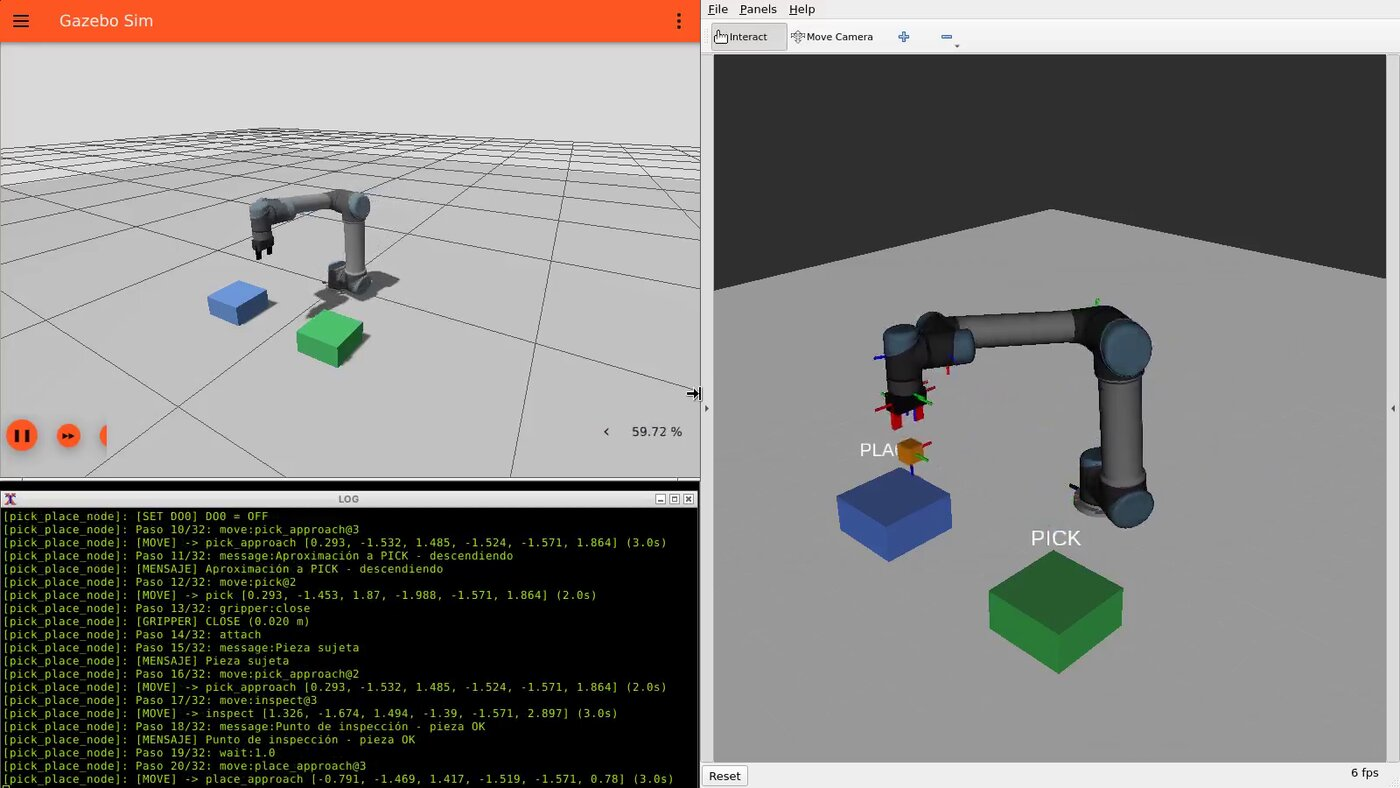
\includegraphics[width=0.75\linewidth]{pp_frame.jpg}\\[1cm]
  {\large \fecha}
\end{titlepage}

\tableofcontents
\newpage

% ============================ ENLACES ============================
\section{Enlaces de entrega}

\begin{itemize}[leftmargin=*]
  \item \textbf{Repositorio de la solución} (incluye el nodo Pick \& Place):\\
        \url{\repo}
  \item \textbf{Nodo Pick \& Place} (paquete \texttt{ur5\_pick\_place}):\\
        \url{\repotree/src/ur5_pick_place}
  \item \textbf{Paquete generado con el MoveIt Setup Assistant} (\texttt{ur5\_robotiq\_moveit\_config}):\\
        \url{\repotree/src/ur5_robotiq_moveit_config}
  \item \textbf{Nodo que ejecuta trayectorias con MoveIt} (\texttt{ur5\_moveit\_executor}):\\
        \url{\repotree/src/ur5_moveit_executor}
  \item \textbf{Paquetes base}: \url{https://github.com/DanielPalominoS/ur5_gripper_packages}
\end{itemize}

\begin{table}[H]
\centering
\caption{Videos de evidencia (carpeta \texttt{media/videos} del repositorio).}
\label{tab:videos}
\begin{tabularx}{\linewidth}{@{}l X r@{}}
\toprule
Video & Contenido & Duración \\
\midrule
\href{\repoblob/media/videos/01_control_por_topicos.mp4}{\texttt{01\_control\_por\_topicos}} & Actividad 1: identificación de controladores y tópicos; brazo y gripper comandados con \texttt{ros2 topic pub}. & 1:13 \\
\href{\repoblob/media/videos/02_pick_and_place.mp4}{\texttt{02\_pick\_and\_place}} & Actividad 2: dos ciclos de la rutina Pick \& Place con E/S digitales simuladas (Gazebo, RViz y log). & 1:59 \\
\href{\repoblob/media/videos/03_setup_assistant_pasos.mp4}{\texttt{03\_setup\_assistant\_pasos}} & Actividad 3: pasos de configuración en el MoveIt Setup Assistant. & 1:00 \\
\href{\repoblob/media/videos/04a_moveit_rviz_error_aceleracion.mp4}{\texttt{04a\_moveit\_rviz\_error\_aceleracion}} & Actividad 3: falla inicial de planificación (límites de aceleración). & 0:32 \\
\href{\repoblob/media/videos/04_moveit_rviz_planificacion.mp4}{\texttt{04\_moveit\_rviz\_planificacion}} & Actividad 3: planificación y ejecución de los grupos \texttt{ur\_arm} y \texttt{gripper} con el plugin de MoveIt en RViz. & 1:03 \\
\href{\repoblob/media/videos/05_moveit_executor_gazebo.mp4}{\texttt{05\_moveit\_executor\_gazebo}} & Actividad 4: nodo MoveItPy ejecutando trayectorias en Gazebo y esquivando un obstáculo. & 0:32 \\
\bottomrule
\end{tabularx}
\end{table}

% ============================ INTRODUCCIÓN ============================
\section{Objetivos}

\begin{enumerate}[leftmargin=*]
  \item Construir los paquetes de simulación del UR5 con gripper en un \emph{workspace} local y controlar el brazo y el gripper mediante comandos publicados en ROS.
  \item A partir de los tópicos identificados, desarrollar un paquete con un nodo que simule una rutina \emph{Pick \& Place} con al menos tres puntos de interés y, en ellos, operaciones de apertura y cierre del gripper, mensajes informativos, espera de entradas digitales y activación de salidas digitales.
  \item Generar con el \emph{MoveIt Setup Assistant} un paquete de configuración de MoveIt para el robot con gripper, documentarlo y verificarlo planificando trayectorias en RViz.
  \item Usar esa configuración para ejecutar trayectorias desde un nodo del ecosistema MoveIt.
\end{enumerate}

% ============================ ENTORNO ============================
\section{Entorno y metodología}

La solución se desarrolló sobre \textbf{ROS~2 Jazzy}, \textbf{Gazebo Harmonic} y \textbf{MoveIt~2.12}. La Tabla~\ref{tab:entorno} resume las versiones. Como no fue posible instalar ROS~2 desde \texttt{packages.ros.org} en el equipo de ejecución (hallazgo H1), se utilizó la distribución \textbf{RoboStack} (conda-forge), que empaqueta las mismas versiones de ROS~2 Jazzy. La simulación se ejecutó en Ubuntu 24.04 sin GPU, con render por software (Mesa \emph{llvmpipe}) sobre una pantalla virtual, desde la que se grabaron los videos. El repositorio incluye \emph{scripts} para reproducir todo en Ubuntu~24.04 / WSL2 con la instalación estándar por \texttt{apt}.

Todos los resultados reportados se verificaron ejecutando la simulación; los \emph{logs} completos se encuentran en \texttt{docs/logs}.

\begin{table}[H]
\centering
\caption{Entorno de software.}
\label{tab:entorno}
\begin{tabular}{@{}ll@{}}
\toprule
Componente & Versión \\
\midrule
Sistema operativo & Ubuntu 24.04 (x86\_64, 2 núcleos, 8 GB RAM, sin GPU) \\
ROS 2 & Jazzy (\texttt{ros-jazzy-desktop} 0.11, RoboStack) \\
Gazebo & Harmonic (\texttt{ros\_gz} 1.0.24, \texttt{gz\_ros2\_control} 1.2.20) \\
MoveIt 2 & 2.12.4 (\texttt{moveit}, \texttt{moveit\_py}, \texttt{moveit\_setup\_assistant}) \\
Universal Robots & \texttt{ur\_description} 3.3, \texttt{ur\_controllers} 3.9 \\
\bottomrule
\end{tabular}
\end{table}

\paragraph{Estructura del repositorio.} La raíz del repositorio es el \emph{workspace} de \texttt{colcon}:

\begin{lstlisting}
ur5_ros2_moveit_lab/
  src/ur5_gripper_packages/       paquetes base (description + bringup), sin modificar
  src/ur5_pick_place/             Actividad 2: rutina Pick & Place + E/S simuladas
  src/ur5_robotiq_moveit_config/  Actividad 3: salida del MoveIt Setup Assistant
  src/ur5_moveit_executor/        Actividad 4: nodo MoveItPy
  scripts/  docs/  media/videos/  reporte/
\end{lstlisting}

\paragraph{Compilación.}
\begin{lstlisting}[language=bash]
bash scripts/instalar_dependencias.sh   # apt + rosdep
bash scripts/compilar.sh                # colcon build (sin --symlink-install, ver H2)
source scripts/entorno.sh
\end{lstlisting}

% ============================ ACTIVIDAD 1 ============================
\section{Actividad 1: simulación y control por tópicos}

Se compilaron \texttt{ur5\_robotiq\_description} (ament\_cmake) y \texttt{ur5\_robotiq\_bringup} (ament\_python) y se lanzó \texttt{sim\_gz\_sgb.launch.py}, que inicia Gazebo, \texttt{robot\_state\_publisher}, el puente \texttt{/clock} y los controladores de \texttt{ros2\_control}. La expansión del modelo con \texttt{xacro} y \texttt{check\_urdf} confirmó la cadena cinemática \texttt{world} $\rightarrow$ \texttt{base\_link\_parent} $\rightarrow \dots \rightarrow$ \texttt{tool0} $\rightarrow$ \{\texttt{gripper\_base\_link}, \texttt{tool0\_tcp}\}, donde \texttt{tool0\_tcp} está 15~cm delante de la brida.

Con \texttt{ros2 control list\_controllers}, \texttt{ros2 topic list} y \texttt{ros2 action list} se identificaron las interfaces de la Tabla~\ref{tab:interfaces}.

\begin{table}[H]
\centering
\caption{Interfaces de control identificadas.}
\label{tab:interfaces}
\small
\begin{tabularx}{\linewidth}{@{}l >{\raggedright\arraybackslash}X >{\raggedright\arraybackslash}p{4.6cm}@{}}
\toprule
Elemento & Interfaz & Tipo \\
\midrule
Brazo & \texttt{/scaled\_joint\_trajectory\_controller/\allowbreak joint\_trajectory} & \texttt{trajectory\_msgs/\allowbreak JointTrajectory} \\
Brazo & \texttt{/scaled\_joint\_trajectory\_controller/\allowbreak follow\_joint\_trajectory} & acción \texttt{FollowJointTrajectory} \\
Gripper & \texttt{/gripper\_controller/commands} & \texttt{std\_msgs/\allowbreak Float64MultiArray} \\
Estado & \texttt{/joint\_states} & \texttt{sensor\_msgs/JointState} \\
\bottomrule
\end{tabularx}
\end{table}

\noindent Controladores activos:
\begin{itemize}[leftmargin=*,nosep]
  \item \texttt{joint\_state\_broadcaster};
  \item \texttt{scaled\_joint\_trajectory\_controller} (\path{ur_controllers/ScaledJointTrajectoryController});
  \item \texttt{gripper\_controller} (\path{position_controllers/JointGroupPositionController}), dos prismáticas de 0.002 a 0.042~m.
\end{itemize}
Ejemplos de comandos utilizados:

\begin{lstlisting}[language=bash]
ros2 topic pub --once /scaled_joint_trajectory_controller/joint_trajectory \
  trajectory_msgs/msg/JointTrajectory "{joint_names: ['shoulder_pan_joint',
  'shoulder_lift_joint','elbow_joint','wrist_1_joint','wrist_2_joint','wrist_3_joint'],
  points: [{positions: [0.8, -1.2, 1.4, -1.77, -1.57, 0.0], time_from_start: {sec: 3}}]}"
ros2 topic pub --once /gripper_controller/commands std_msgs/msg/Float64MultiArray "{data: [0.004, 0.004]}"
\end{lstlisting}

\noindent La lectura de \texttt{/joint\_states} tras cada comando coincidió con las posiciones enviadas (error $<10^{-9}$~rad en estado estacionario).

\begin{figure}[H]
\centering
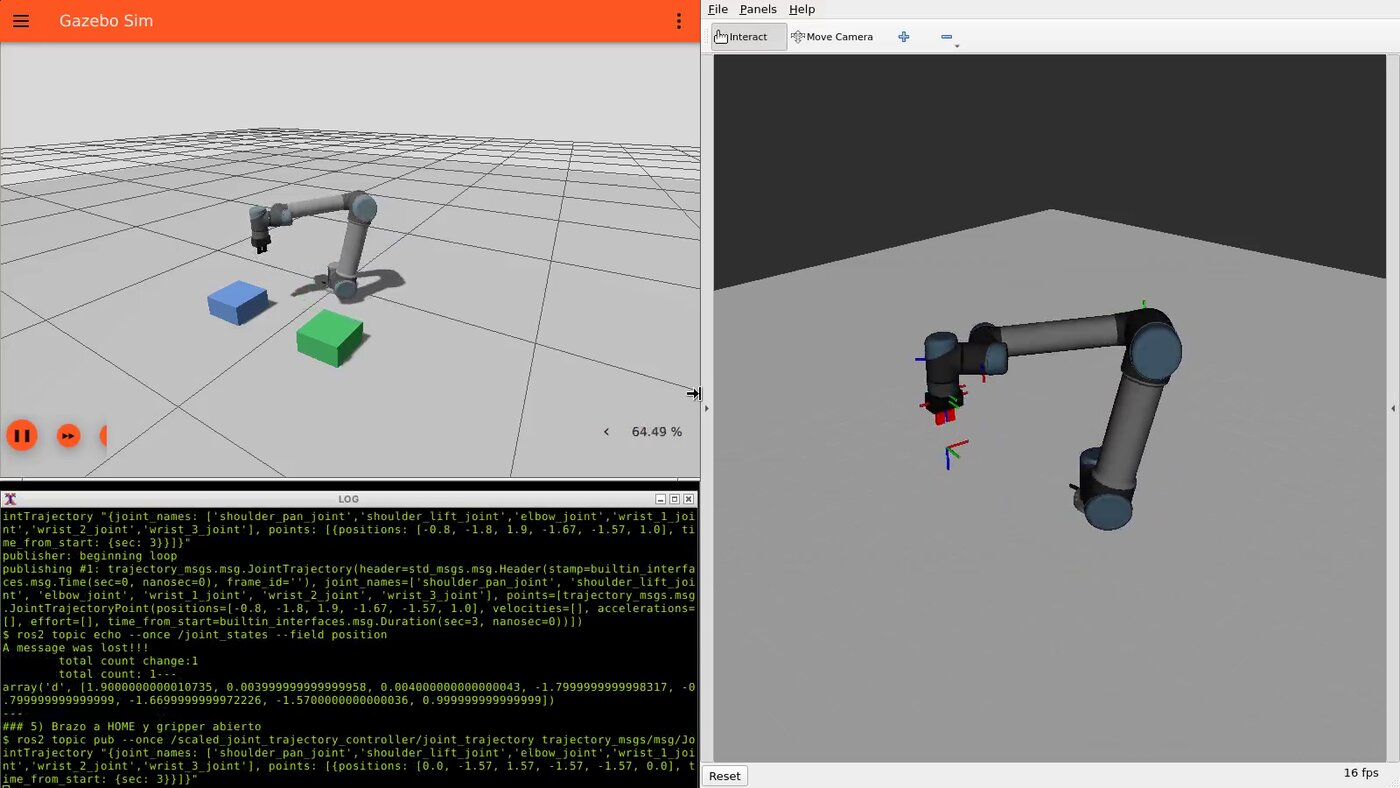
\includegraphics[width=0.95\linewidth]{man_frame.jpg}
\caption{Control por tópicos: Gazebo (izq.), terminal con los comandos y lectura de \texttt{/joint\_states}, y RViz (der.).}
\label{fig:act1}
\end{figure}

% ============================ ACTIVIDAD 2 ============================
\section{Actividad 2: rutina Pick \& Place}

\subsection{Diseño}
El paquete \texttt{ur5\_pick\_place} contiene dos nodos y un \emph{launch} que reutiliza el bringup del repositorio base con un mundo propio (estaciones PICK en verde y PLACE en azul):

\begin{itemize}[leftmargin=*]
  \item \textbf{\texttt{digital\_io\_sim}} -- simula el módulo de E/S de un controlador de robot o PLC con interfaces estándar de ROS~2: cada entrada y salida es un tópico \texttt{std\_msgs/Bool} con QoS \emph{transient local} (\texttt{/io/di0..3}, \texttt{/io/do0..3}) y se modifica con un servicio \texttt{std\_srvs/SetBool} (\texttt{/io/di<n>/set}, \texttt{/io/do<n>/set}). Con \texttt{auto\_cell:=true} emula la lógica de la celda; con \texttt{auto\_cell:=false} las entradas se activan manualmente con \texttt{ros2 service call}.
  \item \textbf{\texttt{pick\_place\_node}} -- intérprete de una rutina declarada en YAML. Mueve el brazo con la acción \texttt{FollowJointTrajectory} (espera el resultado; opcionalmente usa el tópico), acciona el gripper por \texttt{/gripper\_controller/commands} verificando el resultado en \texttt{/joint\_states}, publica mensajes en \texttt{/pick\_place/status}, espera entradas, activa salidas y publica marcadores para RViz.
\end{itemize}

\begin{table}[H]
\centering
\caption{Señales digitales simuladas.}
\label{tab:io}
\begin{tabularx}{\linewidth}{@{}l l X@{}}
\toprule
Señal & Significado & Lógica automática de la celda \\
\midrule
DO0 & Banda transportadora & ON $\Rightarrow$ a los 2~s DI0 = ON \\
DI0 & Pieza presente en PICK & la activa la banda (o el operador) \\
DI2 & Zona de descarga libre & inicia en ON \\
DO1 & Pieza depositada (aviso al PLC) & ON $\Rightarrow$ a los 1.5~s DI1 = ON y DI0 = OFF \\
DI1 & Confirmación del PLC & la activa la lógica (o el operador) \\
\bottomrule
\end{tabularx}
\end{table}

\subsection{Puntos de interés y operaciones}
Los puntos se calcularon por cinemática inversa (parámetros DH del UR5, herramienta hacia abajo) y se verificaron en Gazebo con \texttt{tf2\_echo world tool0\_tcp} (p.~ej. \texttt{pick} $\rightarrow$ (0.450, 0.250, 0.120)~m, exacto). La Tabla~\ref{tab:puntos} resume las operaciones realizadas en cada punto.

\begin{table}[H]
\centering
\caption{Puntos de interés de la rutina y operaciones.}
\label{tab:puntos}
\begin{tabularx}{\linewidth}{@{}l c X@{}}
\toprule
Punto & TCP $(x,y,z)$ [m] & Operaciones \\
\midrule
\texttt{home} & (0.49, 0.11, 0.28) & mensaje, abrir gripper, \textbf{activar DO0}, \textbf{esperar DI0}, desactivar DO0 \\
\texttt{pick\_approach} & (0.45, 0.25, 0.30) & mensaje \\
\texttt{pick} & (0.45, 0.25, 0.12) & \textbf{cerrar gripper}, mensaje ``Pieza sujeta'' \\
\texttt{inspect} & (0.00, 0.45, 0.35) & mensaje, pausa \\
\texttt{place\_approach} & (0.45, $-$0.30, 0.30) & mensaje, \textbf{esperar DI2} \\
\texttt{place} & (0.45, $-$0.30, 0.12) & \textbf{abrir gripper}, \textbf{activar DO1}, \textbf{esperar DI1}, desactivar DO1 \\
\bottomrule
\end{tabularx}
\end{table}

Fragmento de la rutina (\texttt{config/pick\_place\_routine.yaml}):
\begin{lstlisting}
step_list:
  - "move:pick@2"
  - "gripper:close"
  - "message:Pieza sujeta"
  - "move:place_approach@3"
  - "wait_input:2=ON"
  - "move:place@2"
  - "gripper:open"
  - "set_output:1=ON"
  - "wait_input:1=ON"
\end{lstlisting}

\subsection{Resultados}
Se ejecutaron dos ciclos completos sin errores: 18 movimientos del brazo, 6 operaciones del gripper, 8 cambios de salidas digitales y 6 esperas de entradas satisfechas (log \texttt{docs/logs/pick\_place\_run.log}). En RViz la pieza (cubo naranja) aparece en PICK al activarse DI0, se adjunta al TCP al cerrar el gripper y queda en PLACE al abrirlo.

\begin{figure}[H]
\centering
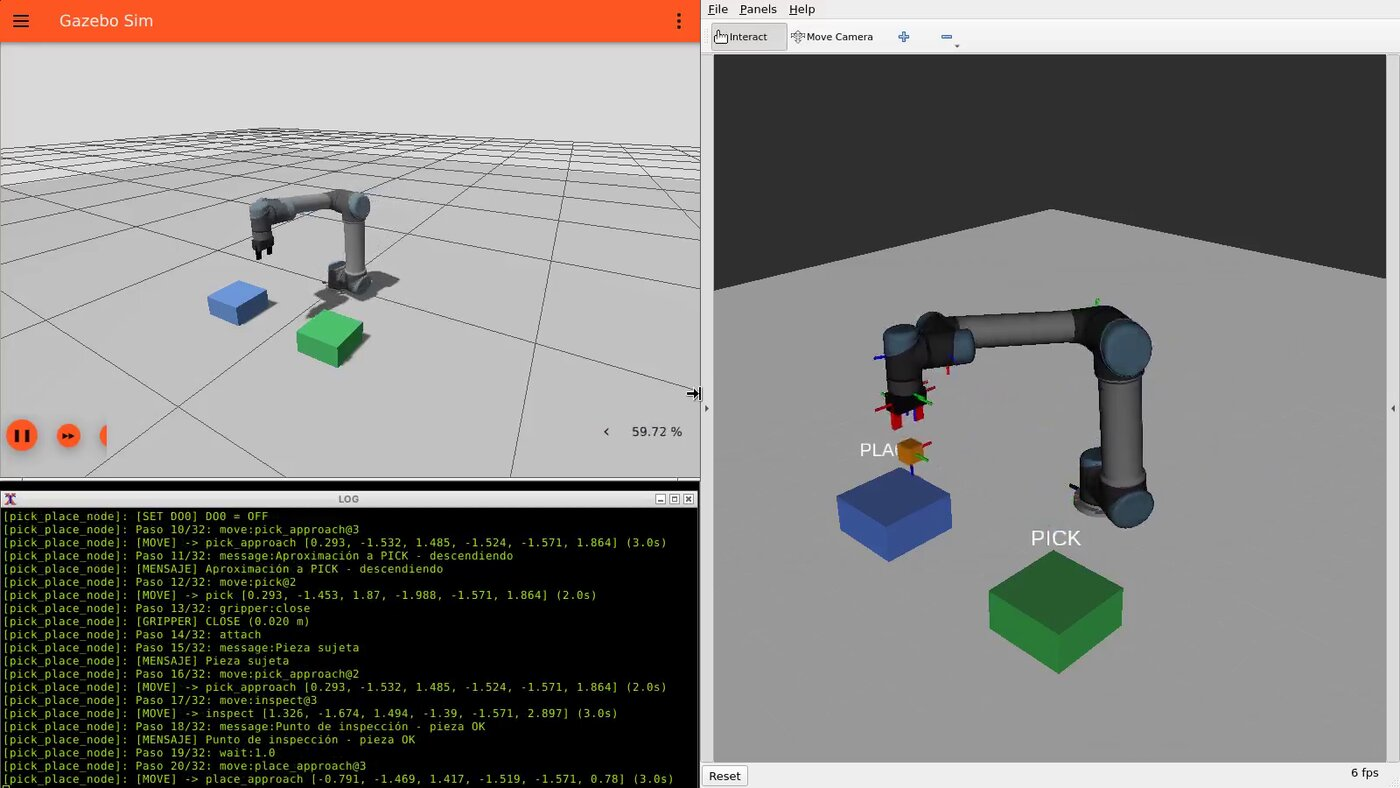
\includegraphics[width=0.95\linewidth]{pp_frame.jpg}
\caption{Pick \& Place: Gazebo con las estaciones (izq.), log de la rutina (abajo) y RViz con la pieza sujeta camino a PLACE (der.).}
\label{fig:pp}
\end{figure}

\begin{lstlisting}
[MENSAJE] Encendiendo banda transportadora (DO0)
[SET DO0] DO0 = ON
[WAIT DI0] esperando ON ...
[digital_io_sim]: DI0: OFF->ON
[WAIT DI0] condición cumplida
[MOVE] -> pick [0.293, -1.453, 1.87, -1.988, -1.571, 1.864] (2.0s)
[GRIPPER] CLOSE (0.020 m)
[MENSAJE] Pieza sujeta
\end{lstlisting}

% ============================ ACTIVIDAD 3 ============================
\section{Actividad 3: paquete MoveIt con el Setup Assistant}

\subsection{Configuración}
Se siguió la guía \texttt{MoveitSetupAssConfig.md} del repositorio base con la interfaz gráfica del asistente. La Tabla~\ref{tab:msa} resume cada paso y la Figura~\ref{fig:msa} muestra capturas; el video \texttt{03\_setup\_assistant\_pasos} recorre todas las pantallas. La salida del asistente se guardó sin cambios en un \emph{commit} propio, y las correcciones posteriores (H8--H9) en otro, para que sean trazables.

\begin{table}[H]
\centering
\caption{Configuración realizada en el MoveIt Setup Assistant.}
\label{tab:msa}
\begin{tabularx}{\linewidth}{@{}l X@{}}
\toprule
Pantalla & Configuración \\
\midrule
Start Screen & Nuevo paquete desde \texttt{ur\_with\_gripper\_moveit.urdf.xacro} \\
Self-Collisions & Matriz generada con valores por defecto: 19 pares deshabilitados \\
Virtual Joints & Ninguno: el URDF ya fija \texttt{world}$\rightarrow$\texttt{base\_link\_parent} (H6) \\
Planning Groups & \texttt{ur\_arm}: KDL, RRTConnect, 6 revolutas; \texttt{gripper}: sin solver, 2 prismáticas \\
Robot Poses & \texttt{home}, \texttt{ready} (\texttt{ur\_arm}); \texttt{open} (0.04), \texttt{close} (0.004) (\texttt{gripper}) \\
End Effectors & \texttt{arm\_eef}: grupo \texttt{gripper}, \emph{parent link} \texttt{tool0} (H7) \\
ros2\_control URDF & comando \texttt{position}; estado \texttt{position}, \texttt{velocity} \\
ROS 2 Controllers & \texttt{scaled\_joint\_trajectory\_controller} (JointTrajectoryController), \texttt{gripper\_controller} (GripperActionController) \\
MoveIt Controllers & \texttt{scaled\_joint\_trajectory\_controller} (FollowJointTrajectory, por defecto), \texttt{gripper\_controller} (GripperCommand) \\
Configuration Files & Salida en \texttt{src/ur5\_robotiq\_moveit\_config} \\
\bottomrule
\end{tabularx}
\end{table}

\begin{figure}[H]
\centering
\begin{subfigure}{0.49\linewidth}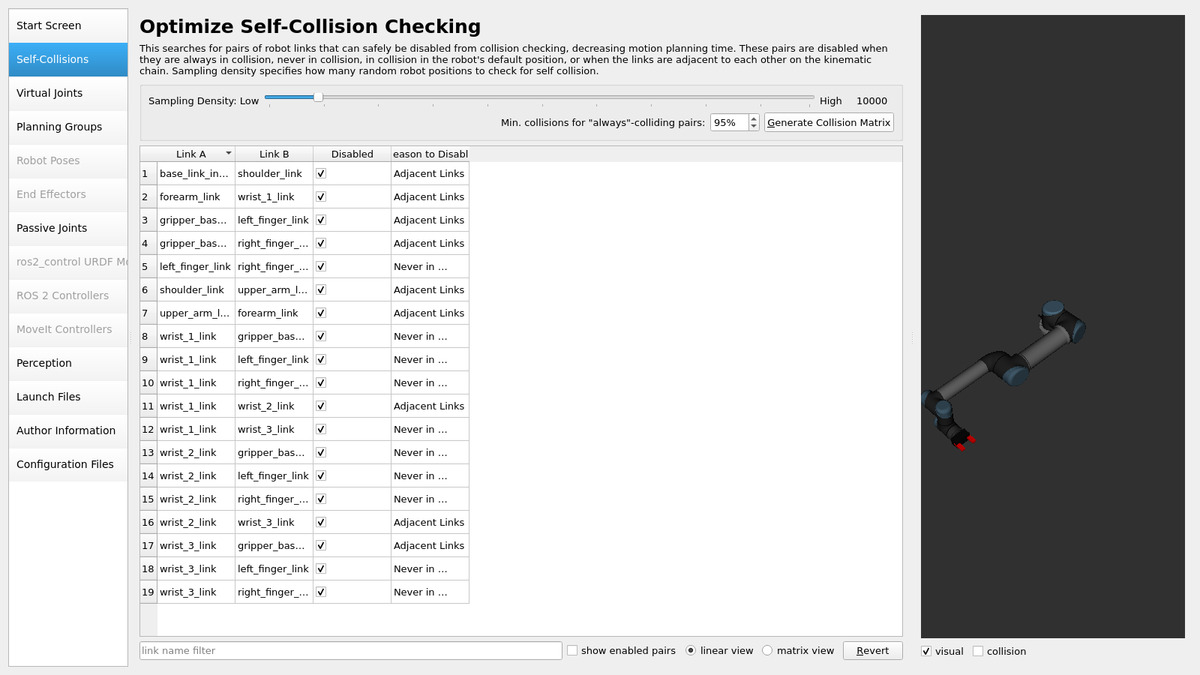
\includegraphics[width=\linewidth]{03_self_collisions.jpg}\caption{Self-Collisions}\end{subfigure}
\begin{subfigure}{0.49\linewidth}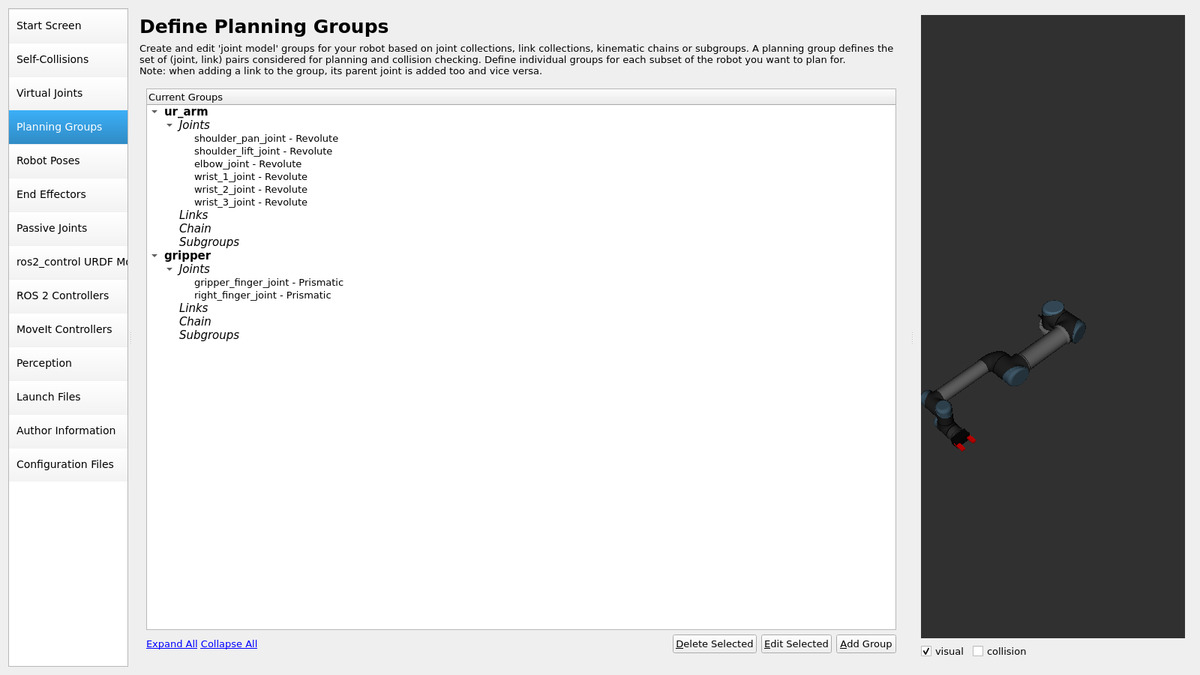
\includegraphics[width=\linewidth]{08_planning_groups.jpg}\caption{Planning Groups}\end{subfigure}\\[4pt]
\begin{subfigure}{0.49\linewidth}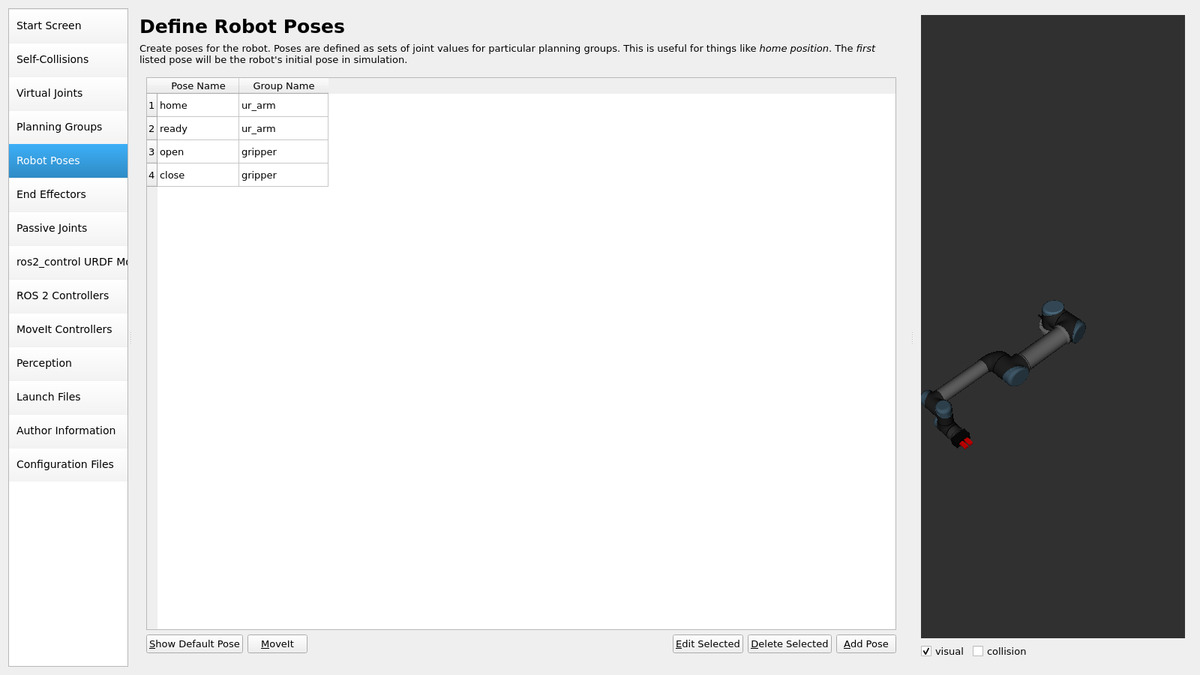
\includegraphics[width=\linewidth]{12_poses.jpg}\caption{Robot Poses}\end{subfigure}
\begin{subfigure}{0.49\linewidth}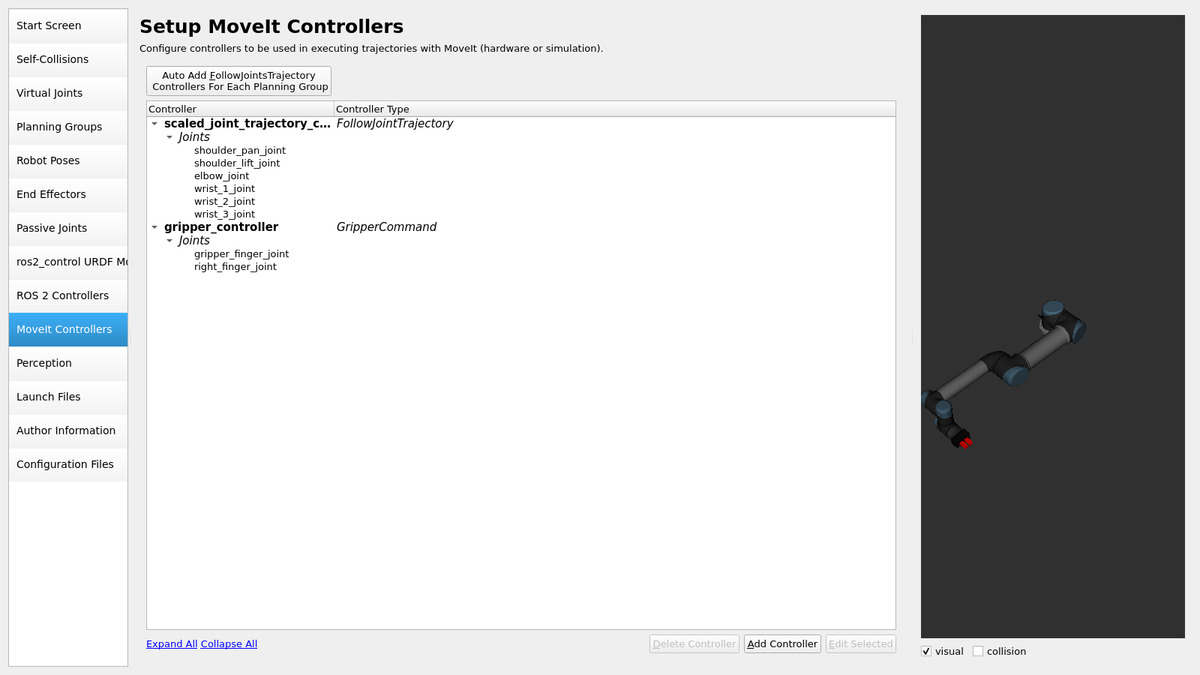
\includegraphics[width=\linewidth]{17_moveit_controllers.jpg}\caption{MoveIt Controllers}\end{subfigure}\\[4pt]
\begin{subfigure}{0.49\linewidth}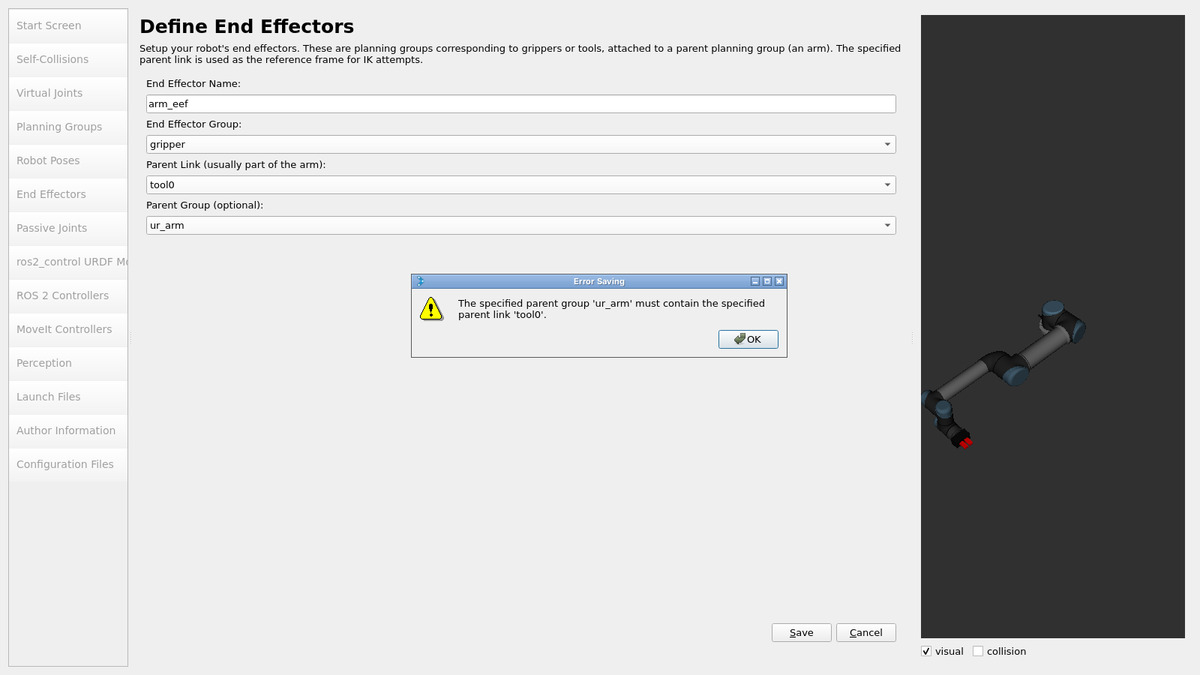
\includegraphics[width=\linewidth]{13b_eef_error_parent_group.jpg}\caption{Error del \emph{parent group} (H7)}\end{subfigure}
\begin{subfigure}{0.49\linewidth}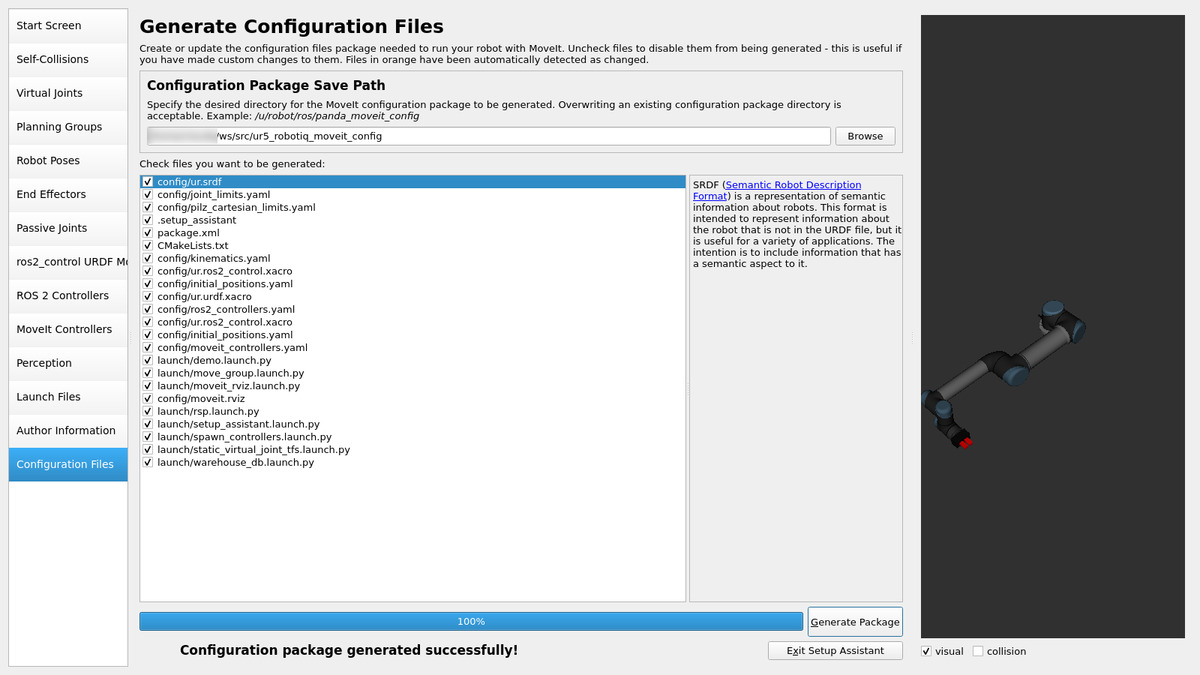
\includegraphics[width=\linewidth]{20_generated.jpg}\caption{Paquete generado}\end{subfigure}
\caption{Capturas del MoveIt Setup Assistant (todas en \texttt{docs/img/msa}).}
\label{fig:msa}
\end{figure}

\subsection{Paquete obtenido}
\begin{table}[H]
\centering
\caption{Archivos principales de \texttt{ur5\_robotiq\_moveit\_config}.}
\begin{tabularx}{\linewidth}{@{}l X@{}}
\toprule
Archivo & Contenido \\
\midrule
\texttt{config/ur.srdf} & grupos, estados con nombre, efector final y colisiones deshabilitadas \\
\texttt{config/kinematics.yaml} & \texttt{ur\_arm} $\rightarrow$ \texttt{KDLKinematicsPlugin} \\
\texttt{config/joint\_limits.yaml} & límites de velocidad y aceleración (corregido, H8) \\
\texttt{config/ros2\_controllers.yaml} & controladores del sistema simulado del demo \\
\texttt{config/moveit\_controllers.yaml} & controladores que MoveIt usa para ejecutar \\
\texttt{config/ur.urdf.xacro}, \texttt{ur.ros2\_control.xacro} & URDF + \texttt{ros2\_control} con \texttt{mock\_components} \\
\texttt{launch/demo.launch.py} & RViz + \texttt{move\_group} + \texttt{ros2\_control} simulado \\
\bottomrule
\end{tabularx}
\end{table}

\subsection{Pruebas de planificación en RViz}
Con \texttt{ros2 launch ur5\_robotiq\_moveit\_config demo.launch.py} se probaron ambos grupos desde el panel \emph{MotionPlanning}. La primera ejecución falló en todas las planificaciones del brazo (``\emph{No acceleration limit was defined for joint shoulder\_pan\_joint}'', H8). Tras habilitar los límites de aceleración, todas las pruebas terminaron con estado \texttt{SUCCEEDED} (Tabla~\ref{tab:rviz}).

\begin{table}[H]
\centering
\caption{Pruebas con el plugin de MoveIt en RViz.}
\label{tab:rviz}
\begin{tabular}{@{}l l l l@{}}
\toprule
Grupo & Meta & Comando & Resultado \\
\midrule
\texttt{ur\_arm} & \texttt{ready} & Plan + Execute & plan en 0.04~s, SUCCEEDED \\
\texttt{ur\_arm} & \texttt{<random valid>} & Plan \& Execute & SUCCEEDED \\
\texttt{ur\_arm} & \texttt{home} & Plan \& Execute & SUCCEEDED \\
\texttt{gripper} & \texttt{close} / \texttt{open} & Plan \& Execute & SUCCEEDED (acción \texttt{gripper\_cmd}) \\
\bottomrule
\end{tabular}
\end{table}

\begin{figure}[H]
\centering
\begin{subfigure}{0.49\linewidth}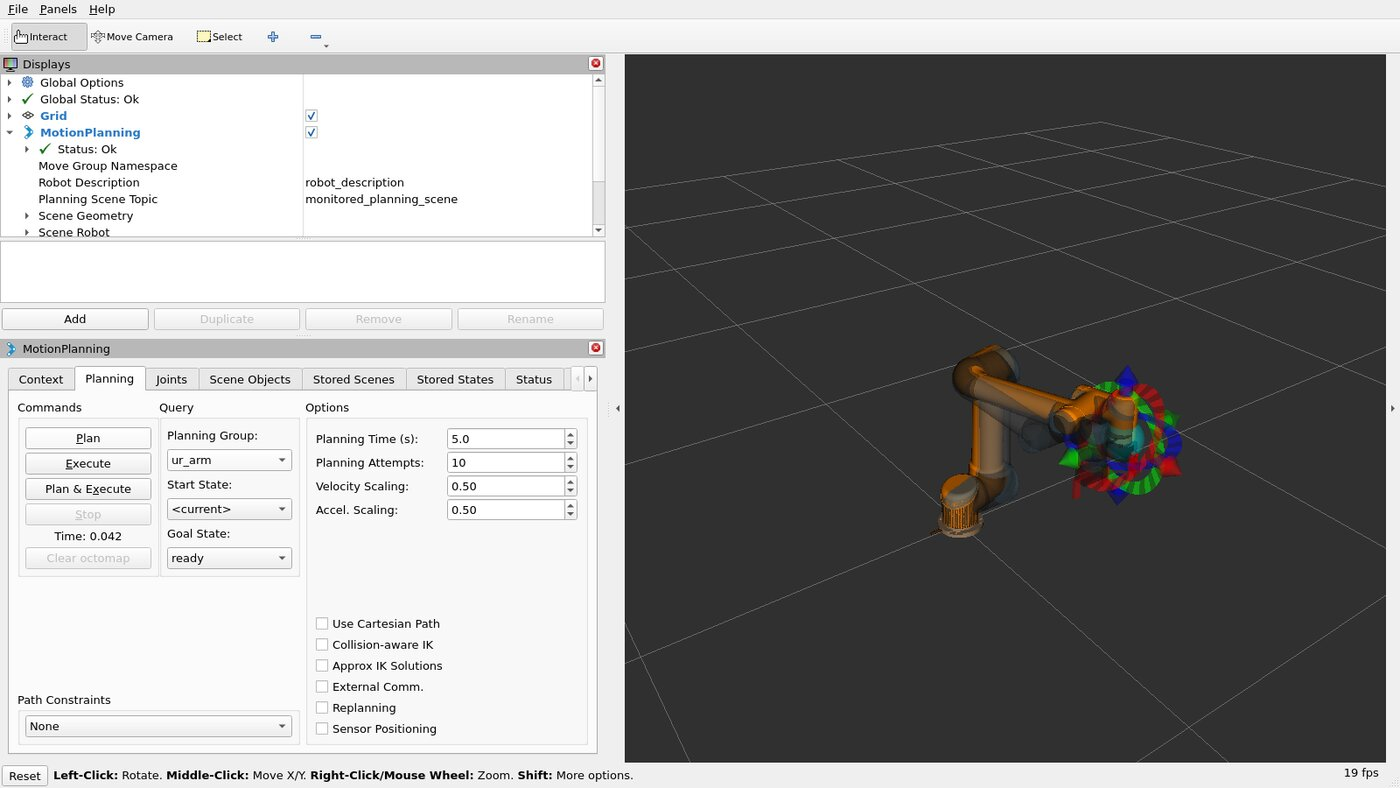
\includegraphics[width=\linewidth]{demo_plan_ready.jpg}\caption{Plan a \texttt{ready} (estado meta en naranja)}\end{subfigure}
\begin{subfigure}{0.49\linewidth}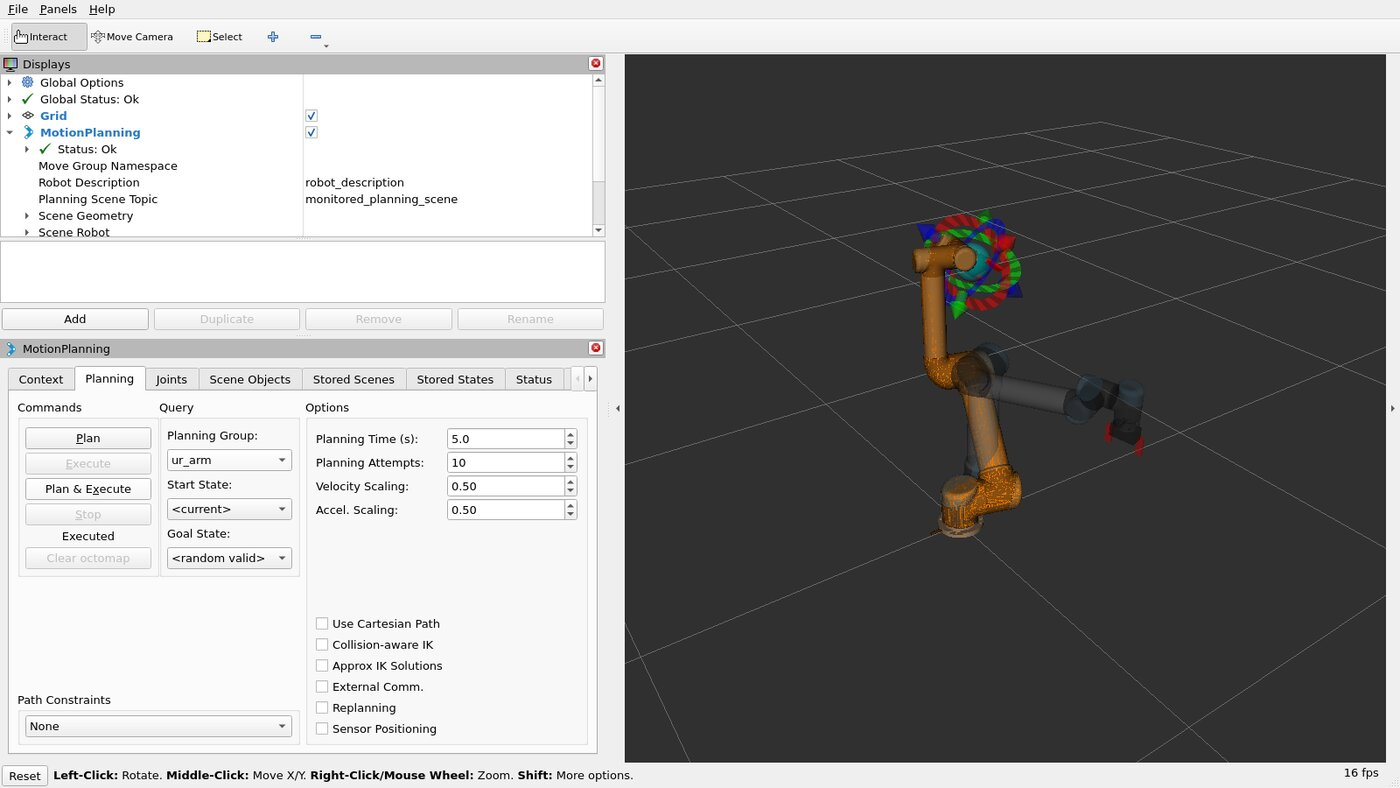
\includegraphics[width=\linewidth]{demo_random_1.jpg}\caption{Meta aleatoria válida}\end{subfigure}
\caption{Planificación con el plugin MotionPlanning de RViz.}
\label{fig:rviz}
\end{figure}

% ============================ ACTIVIDAD 4 ============================
\section{Actividad 4: ejecución de trayectorias con MoveIt}

El paquete \texttt{ur5\_moveit\_executor} lanza Gazebo (bringup base), \texttt{move\_group} con la configuración del asistente (cargada con \texttt{MoveItConfigsBuilder}), RViz y el nodo \texttt{moveit\_executor}, escrito con la API de Python \textbf{MoveItPy}. El nodo:

\begin{enumerate}[leftmargin=*]
  \item planifica al estado \texttt{ready} del SRDF y lo ejecuta;
  \item agrega un obstáculo (``pared'' de $0.30\times0.04\times0.25$~m entre PICK y PLACE) a la \emph{planning scene};
  \item planifica a una pose del TCP sobre PICK con OMPL/RRTConnect;
  \item desciende y sube en línea recta con el planificador \textbf{Pilz LIN};
  \item cierra y abre el gripper (por tópico, ver H10);
  \item planifica hasta PLACE esquivando la pared y regresa a \texttt{home}.
\end{enumerate}

\begin{lstlisting}[language=Python]
self.arm.set_goal_state(pose_stamped_msg=pose_goal(0.45, -0.30, 0.20), pose_link='tool0_tcp')
result = self.arm.plan()
status = self.robot.execute(result.trajectory, controllers=[])   # ExecutionStatus
\end{lstlisting}

\begin{table}[H]
\centering
\caption{Resultados del nodo \texttt{moveit\_executor} en Gazebo.}
\label{tab:exec}
\begin{tabular}{@{}l l c c l@{}}
\toprule
Meta & Planificador & Tiempo de plan & Puntos & Ejecución \\
\midrule
Estado \texttt{ready} & OMPL & 0.06 s & 23 & SUCCEEDED \\
Pose sobre PICK $(0.45, 0.25, 0.25)$ & OMPL & 0.06 s & 7 & SUCCEEDED \\
Descenso a $z=0.12$ & Pilz LIN & 0.01 s & 12 & SUCCEEDED \\
Subida a $z=0.30$ & Pilz LIN & 0.01 s & 15 & SUCCEEDED \\
Pose sobre PLACE (con pared) & OMPL & 0.07 s & 16 & SUCCEEDED \\
Estado \texttt{home} & OMPL & 0.08 s & 14 & SUCCEEDED \\
\bottomrule
\end{tabular}
\end{table}

\begin{figure}[H]
\centering
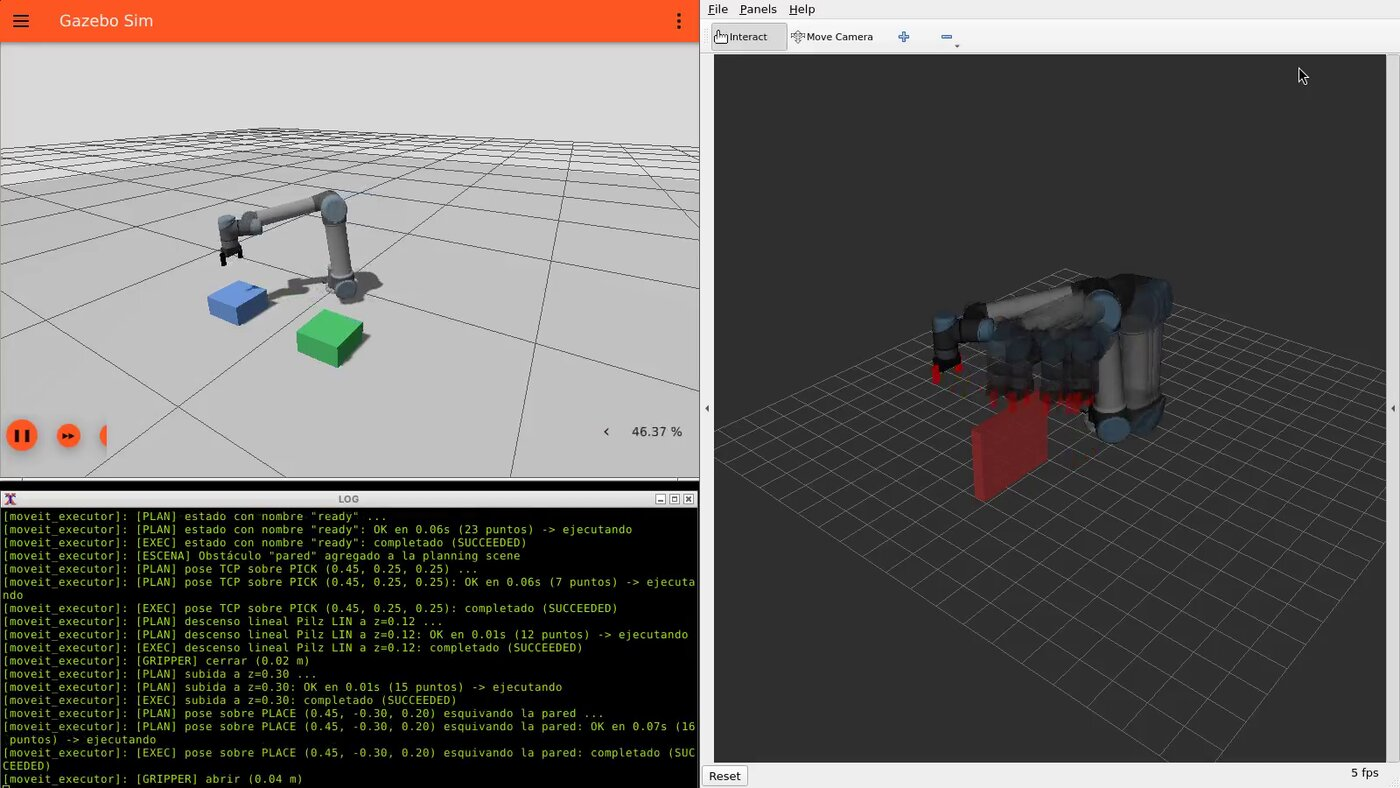
\includegraphics[width=0.95\linewidth]{ex_b.jpg}
\caption{Nodo MoveItPy: el robot en Gazebo (izq.), log del nodo (abajo) y RViz con la pared en la escena de planificación y la trayectoria planificada (der.).}
\label{fig:exec}
\end{figure}

% ============================ HALLAZGOS ============================
\section{Hallazgos, dificultades y alternativas}

El detalle completo, con mensajes de error y \emph{logs}, está en \texttt{docs/hallazgos.md}.

\small
\begin{longtable}{@{}p{0.6cm} >{\raggedright\arraybackslash}p{4.0cm} p{10.6cm}@{}}
\toprule
\# & Problema & Diagnóstico y solución / alternativa \\
\midrule
\endhead
H1 & ROS 2 no instalable desde \texttt{packages.ros.org} & Host inaccesible (DNS/403). Alternativa: RoboStack (conda-forge) con ROS 2 Jazzy, Gazebo y MoveIt; en WSL se documenta la instalación por \texttt{apt}. \\
H2 & \texttt{colcon build --symlink-install} falla & ``\emph{option --editable not recognized}'': setuptools $\geq$ 80 eliminó el modo \texttt{develop}. Se compila sin \texttt{--symlink-install} (o \texttt{setuptools<80}). \\
H3 & \texttt{xacro}: ``\emph{Undefined substitution argument name}'' & El atributo \texttt{name} del robot usa \texttt{\$(arg name)} antes de declararlo; pasar \texttt{name:=ur}. \\
H4 & Tópicos \texttt{/io/di/0} inválidos & En ROS 2 un segmento no puede empezar con dígito; se usó \texttt{/io/di0}. \\
H5 & El Setup Assistant se cierra al escribir la ruta & Recarga el archivo en cada tecla; si la ruta parcial es un directorio lanza \texttt{std::length\_error} y aborta. Solución: pegar la ruta completa o usar \emph{Browse}. \\
H6 & Virtual joint de la guía & El URDF ya define \texttt{world}$\rightarrow$\texttt{base\_link\_parent}; el asistente solo admite el link raíz como hijo. No se agregó. \\
H7 & ``\emph{parent group must contain parent link tool0}'' & \texttt{ur\_arm} (definido por articulaciones) termina en \texttt{wrist\_3\_link}. Se dejó vacío el \emph{parent group}, como en la guía; alternativa: definir el grupo como cadena hasta \texttt{tool0}. \\
H8 & Planificación falla en \path{AddTimeOptimalParameterization} & El asistente genera \texttt{has\_acceleration\_limits: false}; se habilitaron 5~rad/s$^2$ (brazo) y 1~m/s$^2$ (dedos). \\
H9 & Posiciones iniciales fuera de límites & Dedos en 0 con límite inferior 0.002~m; se usó HOME y gripper abierto. \\
H10 & Controlador del gripper & \texttt{GripperActionController} maneja un solo joint; en Gazebo el gripper es un \texttt{JointGroupPositionController} sin acción. MoveIt ejecuta solo el brazo en Gazebo y el gripper se acciona por tópico. Alternativa futura: \texttt{mimic} + controlador de gripper paralelo. \\
H11 & Estado inicial en colisión & En Gazebo el robot arranca con articulaciones en 0, dentro del obstáculo; se mueve a \texttt{ready} antes de insertarlo. \\
H12 & \texttt{execute()} devuelve ABORTED (intermitente) & El cliente de acción aún no estaba conectado; se agregó espera, verificación de \texttt{ExecutionStatus} y reintentos. \\
H13 & Obstáculo invisible en RViz & La escena de MoveItPy es local; se publica un \emph{diff} en \texttt{/planning\_scene}. \\
H14 & Rendimiento sin GPU & RTF de Gazebo 45--65~\% y RViz 3--30~fps con render por software; no afecta los resultados (tiempo de simulación). \\
H15 & Detalles menores & Texto de RViz con espacios separados; clave duplicada en \texttt{.setup\_assistant}; la pieza del Pick \& Place es visual (sin física de agarre; alternativa: plugin \texttt{DetachableJoint}). \\
\bottomrule
\end{longtable}

\normalsize
\paragraph{Fuentes consultadas.} Documentación oficial de MoveIt 2 (tutoriales del Setup Assistant y de MoveItPy), documentación de \texttt{ros2\_control}/\texttt{ros2\_controllers}, la guía \texttt{MoveitSetupAssConfig.md} del repositorio base, y los mensajes de error y el código fuente de los paquetes involucrados.

% ============================ CONCLUSIONES ============================
\section{Conclusiones}

\begin{itemize}[leftmargin=*]
  \item Los controladores de \texttt{ros2\_control} exponen interfaces simples (un tópico de trayectorias y una acción para el brazo, un tópico de posiciones para el gripper) que bastan para programar rutinas industriales sin planificador. Usar la acción \texttt{FollowJointTrajectory} en lugar del tópico permite saber cuándo termina cada movimiento y encadenar operaciones de forma determinista.
  \item Las E/S digitales se pueden simular con tópicos \texttt{Bool} y servicios \texttt{SetBool}, lo que permite probar la lógica de sincronización con la celda (esperas y confirmaciones) antes de tener el hardware, de forma automática o manual.
  \item El MoveIt Setup Assistant genera un paquete funcional en pocos minutos, pero su salida debe revisarse: en MoveIt~2 Jazzy faltan los límites de aceleración y las posiciones iniciales pueden quedar fuera de los límites. Además, la configuración de controladores debe coincidir con la que realmente expone la simulación.
  \item Con MoveItPy se combinan planificadores (OMPL para movimientos libres con evasión de obstáculos y Pilz LIN para aproximaciones rectilíneas), lo que reproduce la forma de programar un ciclo de \emph{pick and place} en un robot real.
\end{itemize}

\end{document}
